\chapter{Μελέτη της Απόδοσης του VQ H.264}
\label{chapter:chap6}

\section{Εισαγωγή}
\label{section:sect61}

\indent Σε αυτό το κεφάλαιο θα παρουσιαστούν και θα αναλυθούν τα αποτελέσματα του VQ H.264, επίσης θα γίνει σύγκριση με τις επιδόσεις του JM H.264. Επίσης θα δειχθεί ότι με την χρήση VQ μπορούμε να βελτιώσουμε την πολυπλοκότητα του decoder σε σχέση με αυτή του JM H.264.

\section{Encoding με VQ H.264}
\label{section:sect62}

\indent Για τις δοκιμές χρησιμοποιήθηκαν 5 βίντεο που δεν είχαν συμπεριληφθεί στο training set και τα στιγμιότυπα τους φαίνονται στο Σχήμα~\ref{fig:testvid}. To PSNR που ο VQ H.264 στα test video φαίνεται στο Σχήμα~\ref{table:testpsnr}.

\begin{table}[h!]
    \begin{center}
        \begin{tabular}{| l | l | l | l |}
        \hline
        Test Video & PSNR I (Y/U/V)dB  & PSNR P (Y/U/V)dB  & PSNR B (Y/U/V)dB       \\ \hline
        test1      & 35.15/39.72/39.67 & 41.16/43.91/43.87 & 43.00/45.14/45.22      \\ \hline
        test2      & 35.51/41.10/42.83 & 38.87/41.53/43.28 & 40.38/43.01/44.71      \\ \hline
        test3      & 30.70/39.86/41.00 & 36.68/42.64/43.76 & 38.00/43.74/44.90      \\ \hline
        test4      & 44.12/47.36/47.91 & 46.00/47.20/47.75 & 46.55/47.42/48.05      \\ \hline
        test5      & 37.01/50.12/48.70 & 44.00/49.90/49.65 & 44.78/50.46/50.29      \\ \hline
        \hline
        \end{tabular}
    \end{center}

    \caption{PSNR των Test videos με κωδικοποίηση στον VQ H.264}
    \label{table:testpsnr}
\end{table}

\begin{figure}[H]
\centering
\begin{tabular}{c c}
    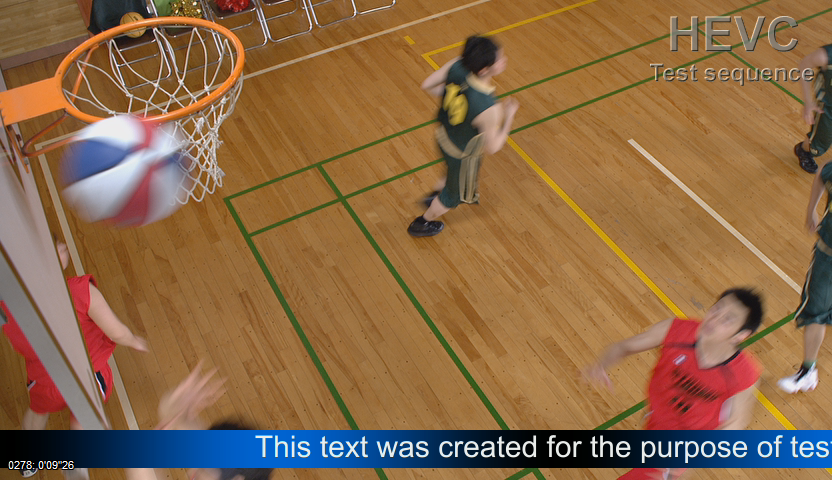
\includegraphics[height=4.0cm]{chapter6/test1.png}
    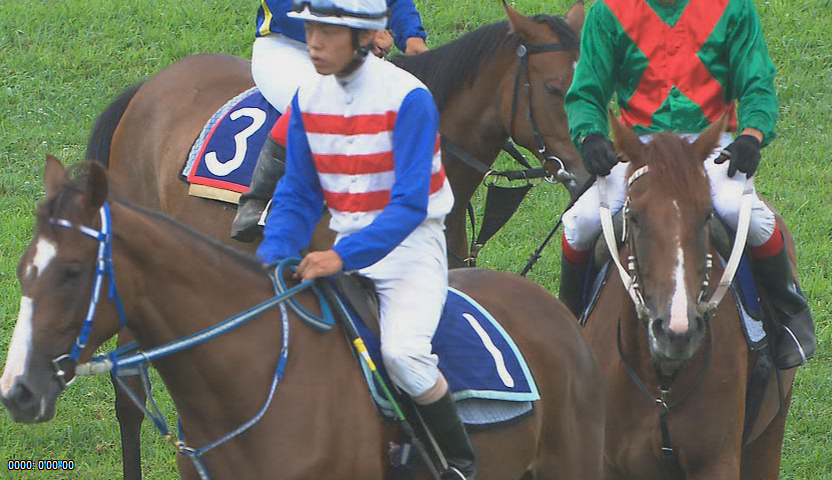
\includegraphics[height=4.0cm]{chapter6/test2.png}\\
    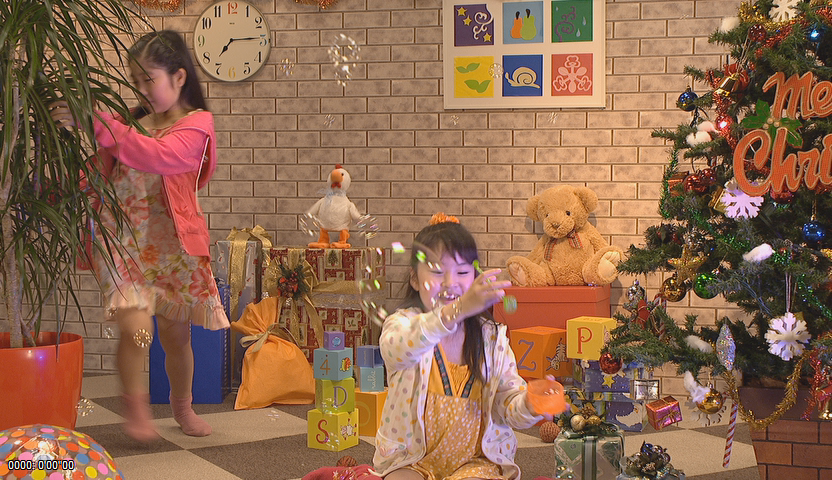
\includegraphics[height=4.0cm]{chapter6/test3.png}
    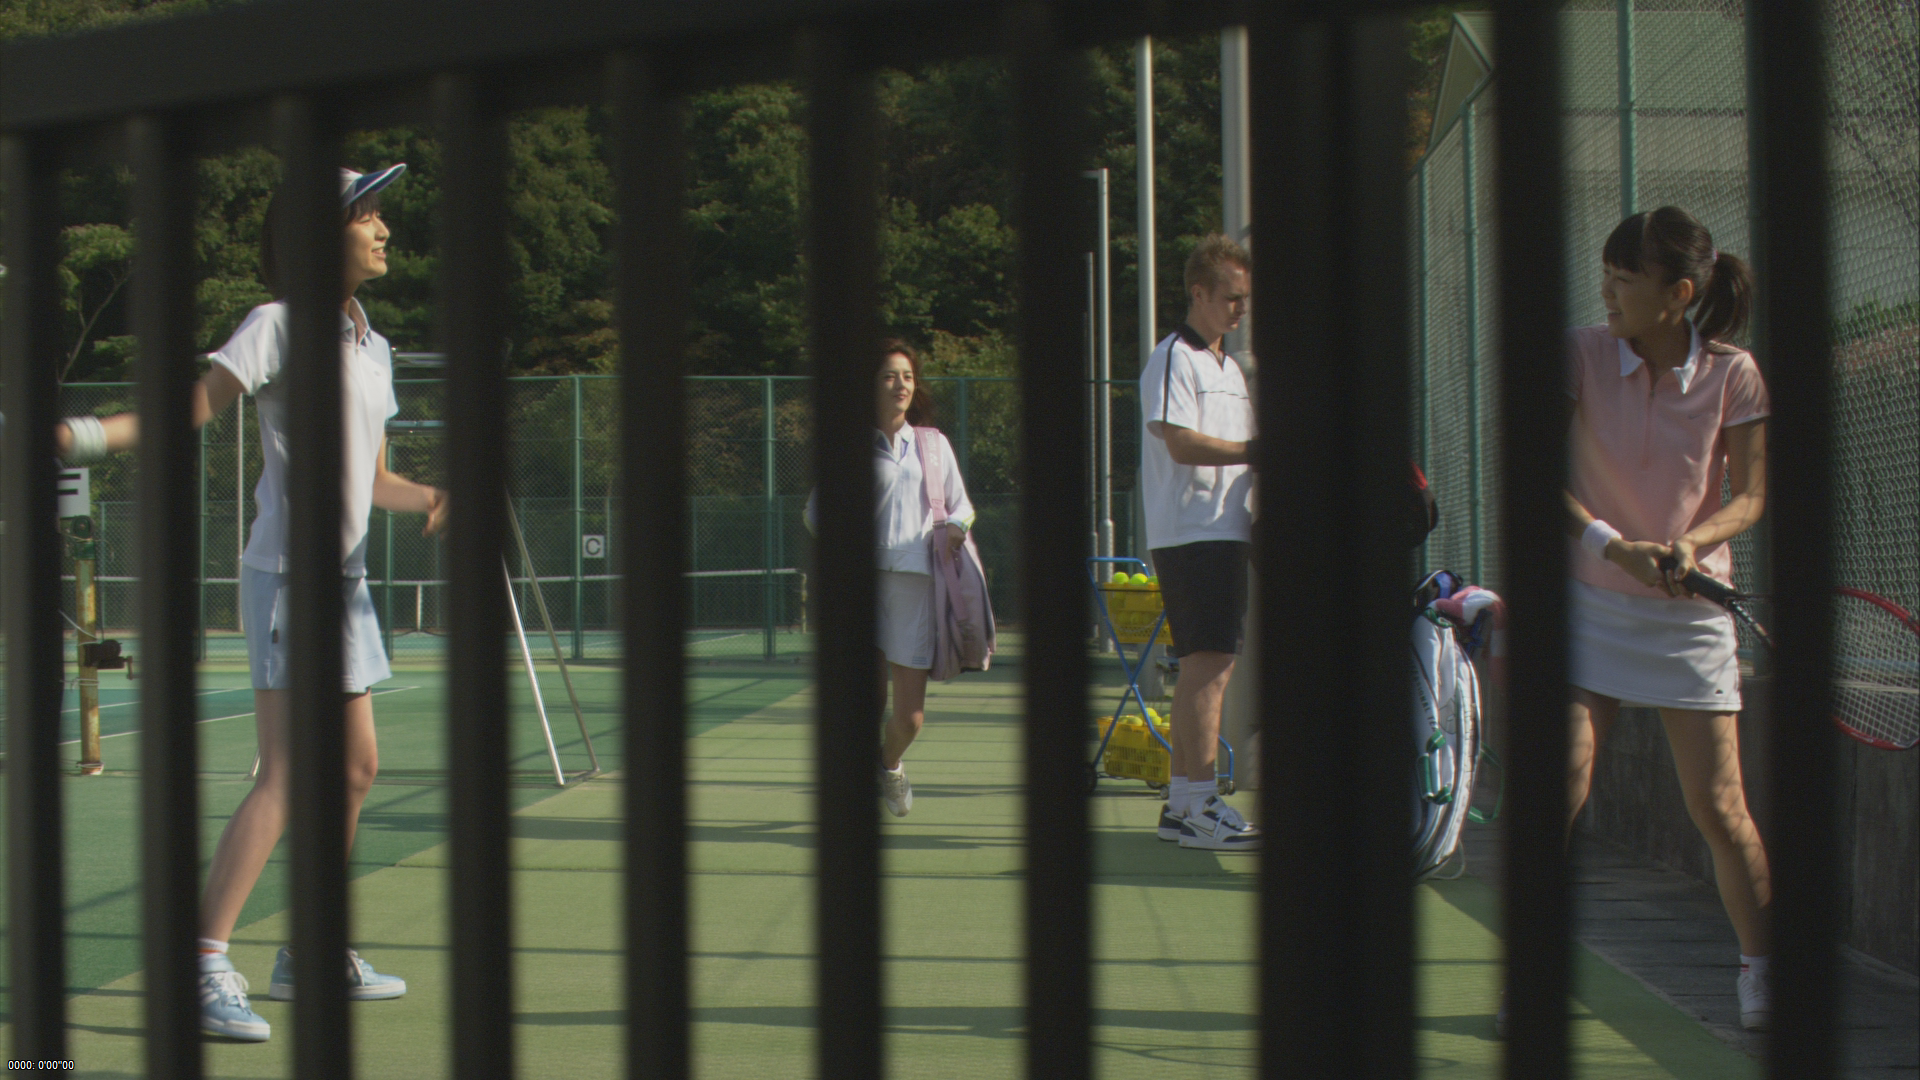
\includegraphics[height=4.0cm]{chapter6/test4.png}\\
    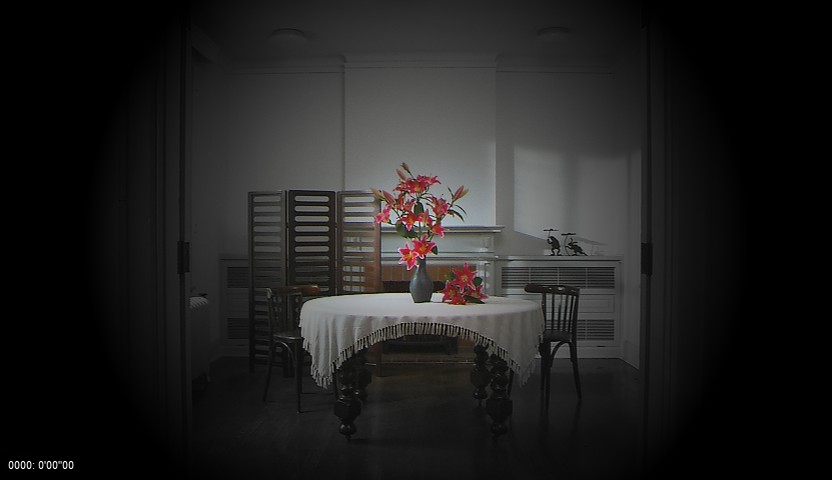
\includegraphics[height=4.0cm]{chapter6/test5.png}
\end{tabular}
\caption{Βίντεο που δοκιμάστηκαν να γίνουν encoding με τον VQ H.264.}
\label{fig:testvid}
\end{figure}

\newpage
\section{Encoding με JM H.264}
\label{section:sect62}

\indent Για να είμαστε σε θέση να συγκρίνουμε τα αποτελέσματα των δύο encoder θα πρέπει να συμπιέσουμε τα ίδια βίντεο με τον JM H.264 με το ίδιο configuration και προσπαθώντας να πετύχουμε τα ίδια PSNR που πέτυχε και ο VQ H.264. Αυτό επιτεύχθηκε δοκιμάζοντας διάφορα QP για τα καρέ I,P,B. Επειδή στον VQ H.264 παρατηρείται ότι το U,V αποδίδει πολύ καλύτερα από το Υ σε κάποια βίντεο χρειάστηκε να υπολογιστεί ο βεβαρημένος μέσος όρος $avg = 0.66*PSNRY+0.16*PSNRU+0.16*PSNRV$ έτσι ώστε να ισχύει $avg_{vq}=avg_{jm}$. Τα αποτελέσματα φαίνονται στον Πίνακα~\ref{table:jm264}.
Η ποσοστιαία διαφορά ως προς τον JM φαίνεται στον Πίνακα~\ref{table:jmvqdiff} και θα την χαρακτήριζα πολύ μικρή έτσι ώστε να έχουμε έγκυρη σύγκριση.

\begin{table}[h!]
    \begin{center}
        \begin{tabular}{| l | l | l | l |}
        \hline
        Test Video & PSNR I (Y/U/V)dB  & PSNR P (Y/U/V)dB  & PSNR B (Y/U/V)dB       \\ \hline
        test1      & 36.31/38.88/38.90 & 42.01/43.95/44.54 & 43.50/44.75/45.49      \\ \hline
        test2      & 37.31/38.43/40.00 & 40.50/41.14/42.24 & 40.50/41.45/42.54      \\ \hline
        test3      & 33.94/37.24/37.85 & 38.64/40.75/41.45 & 38.45/40.51/41.25      \\ \hline
        test4      & 45.18/46.83/47.86 & 45.75/47.13/48.18 & 46.10/47.29/48.21      \\ \hline
        test5      & 39.20/46.76/47.34 & 43.94/47.66/48.28 & 45.14/49.29/49.76      \\ \hline
        \hline
        \end{tabular}
    \end{center}

    \caption{PSNR των Test videos με κωδικοποίηση στον JM H.264}
    \label{table:jm264}
\end{table}

\begin{table}[h!]
    \begin{center}
        \begin{tabular}{| l | l | l | l |}
        \hline
        Test Video & \% Diff I  & \% Diff P & \% Diff B   \\ \hline
        test1      & 1,40	    & -1,40	    & -0,93       \\ \hline
        test2      & 0,83	    & -5,11	    & -4,23       \\ \hline
        test3      & 3,53	    & -5,21	    & -5,49       \\ \hline
        test4      & 1,35	    & -0,87	    & -0,18       \\ \hline
        test5      & 1,69	    & -5,38	    & -2,76       \\ \hline
        \hline
        \end{tabular}
    \end{center}

    \caption{Διαφορές του PSNR JM-VQ. Στα θετικά ο JM είναι καλύτερος από τον VQ ενώ στα αρνητικά το ανάποδο.}
    \label{table:jmvqdiff}
\end{table}

\newpage
\section{VQ H.264 vs JM H.264}
\label{section:sect63}

\indent Για να γίνει η σύγκριση θα υπολογιστούν τα συνολικά bits που ο JM H.264 χρειάστηκε για να αποθηκεύσει τους κβαντοποιημένους συντελεστές του μετασχηματισμού, αυτή η πληροφορία μας παρέχεται απευθείας από την έξοδο του encoder. Αυτό γίνετε γιατί στην ουσία τα $VQ_{indices}$ αντιστοιχούν μόνο στην πληροφορία που μας δίνουν τα residuals, όπως και οι συντελεστές του μετασχηματισμού. Αφού αυτά βρέθηκαν υπολογίστηκε το πλήθος $len(vector_{mode})$ των vectors για κάθε βίντεο και κάθε mode (Intra,Inter) και από το πλήθος αυτών αφαιρούνται 16 vectors για κάθε macroblock που χαρακτηρίζεται από τον encoder σαν skipped. Skipped είναι ένα macroblock για το οποίο ο encoder δε γράφει συντελεστές γιατί είναι όλοι μηδέν. Στο επόμενο βήμα πολλαπλασιάζουμε την εντροπία από τους Πίνακες~\ref{fig:conentropy},~\ref{fig:trainingset} με την διάσταση του VQ για να βρούμε πόσα bits χρειάζονται για κάθε block dxd. Τέλος πολλαπλασιάζουμε τα bits που χρειάζονται ανά block και έχουμε το μέγεθος των $VQ_{indices}$ μετά από συμπίεση. Η αποδόσεις φαίνονται στο Σχήμα~\ref{fig:compare1}.

\begin{figure}[H]
    \centering
    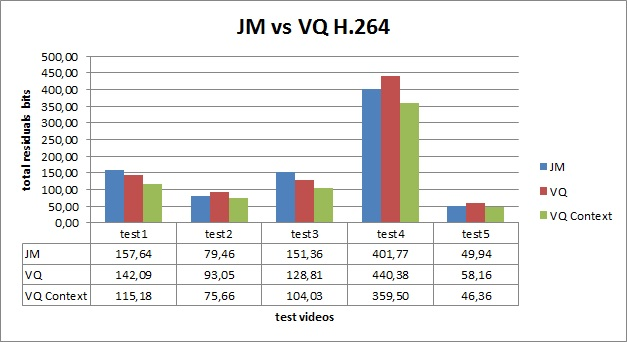
\includegraphics[width=0.8\textwidth]{chapter6/compare1.jpg}
    \caption{Σύγκριση του JM H.264 και VQ H.264 με context entropy και χωρίς context}
    \label{fig:compare1}
\end{figure}